\documentclass[UTF8]{ctexart}
%%%%%%%%%%%%%%%%%%%%%%%%%%%== 引入宏 ==%%%%%%%%%%%%%%%%%%%%%%%%%%%%%
\usepackage{cite}
\usepackage{amsmath}	% 使用数学公式
\usepackage{graphicx}	% 插入图片/PDF/EPS 等图像
\usepackage{subfigure}	% 使用子图像或者子表格
\usepackage{geometry}	% 设置页边距
\usepackage{fancyhdr}	% 设置页眉页脚
\usepackage{setspace}	% 设置行间距
\usepackage{hyperref}	% 让生成的文章目录有链接,点击时会自动跳转到该章节
\usepackage{url}
\usepackage{caption2}
\usepackage{authblk}

\graphicspath{{Figures/}}

%%%%%%%%%%%%%%%%%%%%%%%%%%== 设置全局环境 ==%%%%%%%%%%%%%%%%%%%%%%%%%%%%
% [geometry] 设置页边距
\geometry{top=2.6cm, bottom=2.6cm, left=2.45cm, right=2.45cm, headsep=0.4cm, foot=1.12cm}
% 设置行间距为 1.5 倍行距
\onehalfspacing
% 设置页眉页脚
\pagestyle{fancy}
%\lhead{左头标}
%\chead{\today}
%\rhead{152xxxxxxxx}
\lfoot{}
\cfoot{\thepage}
\rfoot{}
%\renewcommand{\headrulewidth}{0.4pt}
%\renewcommand{\headwidth}{\textwidth}
%\renewcommand{\footrulewidth}{0pt}

%%%%%%%%%%%%%%%%%%%%%%%%%%== 自定义命令  ==%%%%%%%%%%%%%%%%%%%%%%%%%%%%%%
% 此行使文献引用以上标形式显示
\newcommand{\supercite}[1]{\textsuperscript{\cite{#1}}}
% 此行使section中的图、表、公式编号以A-B的形式显示
\renewcommand{\thetable}{\arabic{section}-\arabic{table}}
\renewcommand{\thefigure}{\arabic{section}-\arabic{figure}}
\renewcommand{\theequation}{\arabic{section}-\arabic{equation}}
% 此行使图注、表注与编号之间的分隔符缺省,默认是冒号:
\renewcommand{\captionlabeldelim}{~}

%===================================== 标题设置  ==========================================
% \heiti \kaishu 为字体设置,ctex 会自动根据操作系统加载字体
\title{\huge \CJKfamily{zhhei}基于慕测数据分析学生编程能力}	
\author{侯锐\textsuperscript{1} \quad 吴耀恩\textsuperscript{2} \quad 徐宇轩\textsuperscript{3}}
\affil{\small (\textsuperscript{1}{南京大学软件学院~软件工程~181250xxx}) \\ (\textsuperscript{2}{南京大学软件学院~软件工程~181250xxx}) \\ (\textsuperscript{2}{南京大学软件学院~软件工程~181250xxx})  }	
\date{} % 去除默认日期
%\date{\today}

%===================================== 正文区域  ==========================================
\begin{document}
	\maketitle
	
	\begin{flushleft}
		\textbf{摘要}:利用慕测平台一次编程作业的数据,运用一些数据处理方法,实现对于学生编程能力的评价\\[8pt]
		\textbf{关键词}:PCA,TOPSIS,题目难度,编程能力
	\end{flushleft}
	\section{研究问题}\label{sec1}
	
	\subsection{背景}
	随着人类社会技术的进步,编程逐渐成为信息科学一个基本知识和技能,成为一个跨专业、学科所必备的一个基本素养。很多高校现在更是把编程能力的培养作为理工科学生的必修课,随之流行起来的便是在线测评系统(OJ)。在线测评系统可以保存大量的测评数据,从中我们分析学习者的学习行为。本次研究就是基于慕测平台一次在线作业的数据,对参-+与该次作业的学生的编程能力做一次评价。
	
	\subsection{详细介绍}
	在本次研究中,一方面,我们通过主成分分析法(PCA)对数据中的题目做了分析,得到每个题目的难度系数,将难度系数与参与者对该题目的最终得分相结合,得到学生得分情况的测评;另一方面,我们通过xxxx(侯锐补充)的方法,对参与者提交的代码内容进行分析,得到学生代码书写情况的测评。考虑到不同的学生可能有不同的长处和喜好,分门别类的去评价一个学生的编程能力更加客观,我们针对每个学生,从字符串、树、图、排序等八个角度搜集学生的得分情况和代码情况,通过优劣解距离法(TOPSIS)实现对学生最终编程能力的打分。
	\subsection{应用场景}
	\label{sec1:subsec3}
	通过一次线上作业,老师对每类题型学生的掌握情况做一个大致的了解,方便改进和完善教学方法和促进与学生的沟通。作为学生,在完成一次作业后可以了解到自己与同期学生的差距在哪里,知道自己的优势和短处,有利于后期的学习和提高。
	
	
	\section{研究方法}\label{sec2}
	\subsection{数据集}
	基于慕测平台的提交记录数据,格式是json文件,内容包括每个参与者对每道题目的提交代码、最终得分、每次提交时间、每次提交得分等多个维度数据。通过学生id检索到具体学生,使用pythn提取数据,使用numpy,pandas,sklearn等工具分析。	
	
	\subsection{数据分析方法}
	
	\subsubsection{主成分分析法分析题目难度}
	\par (1)主成分分析法
	\par 主成分分析法也称主分量分析,是把多指标转化为少数几个综合指标,其中每个主成分都能够反映原始变量的大部分信息,主要用于数据降维。其步骤大致分为以下几步:
	\begin{itemize}
		\item 整理原始矩阵$X_{m \times n}$
		\item 求原始矩阵$X_{m \times n}$的协方差矩阵$S_{m \times n}$
		\item 求解协方差阵的特征值和特征向量
		\item 选取最大的$K$(人为给定)个特征值所对应的特征向量组成构成矩阵$W_{n \times k}$
		\item 最后计算$Z_{m \times k}=X_{m \times n}W_{n \times k}$
	\end{itemize}
	\par (2)维度的选取
	\par 根据已有的数据集,先要提取特征集。在提取特征之前,我们首先对数据集中的各个特征之间的关系进行了分析,选择出六个对编程题目难度研究最为有效的特征($X$)。
	\par
	\begin{enumerate}
		\item $X_1$:1A率
		\par 在寻找合适维度的过程中,我们首先考虑到的就是题目的AC数量。我们随机抽取了几道题目,发现不同的题目的AC数量有着较为明显的差异(见图x)。但是我们随即结合自身考虑到这样一种情况,:当一个同学在做练习时,最终运行出正确结果,但他对自己的解法并不满意,即通过了该题但是为了优化解题过程而去多次修改代码并提交通过,这样就提高了AC 量,使得这个特征不能那么客观地反映题目的难度类型。考虑到这个问题,我们最终选取1A率作为第一个维度,即一次通过的比率,用首次提交就通过的人数比总人数。
		\item $X_2$:AC率
		\par 用一道题目的通过人数比上总答题人数
		\item $X_3$:提交次数
		\par 一道题目的答题次数能反映这道题的难度
		\item $X_4$:最终平均分
		\par 每个同学提交成绩的最高分是这个题目的最终分,那么一道题目的最终分数的平均值可以反映这道题目在学生中的大体情况
		\item $X_5$:提交平均分
		\par 同学的每次提交都会得到一个及时反馈,将所有提交分数的均值作为另一个维度能一定程度上反映题目的难度
		\item $X_6$:Debug成效
		\par 部分同学最后一次提交突然变为0然后放弃debug,所以取最终得分而不是最后一次得分,另外也要假定同学做一道题途中不因该题过难而跳过去做另一道题然后过很久再倒回来的情况相对少见,而因题目过难而先跳过去的情况下时间会很长,因而也能反映题目难度。记一位同学最终得分$Score_{final}$,初次提交得分$Score_{first}$,最终提交时间$Time_{final}$,初次提交时间$Time_{first}$,那么
		$$X_6=\frac{Score_{final}-Score_{first}}{Time_{final}-Time_{first}}$$
	\end{enumerate}
	\par (3)数据处理与可视化
	\par 在决定最后保留几个维度的时候,我们首先通过不对n\_components赋值,此时默认返回min(X.shape)个特征,这样虽然没有减少特征个数,但是可以画出累计可解释方差贡献率曲线,以此选择最好的n\_components。累积可解释方差贡献率曲线是一条以降维后保留的特征个数为横坐标,降维后新特征矩阵捕捉到的可解释方差贡献率为纵坐标的曲线,能够帮助我们选择合适的维度。
	\begin{figure}[!htbp]
		\centering
		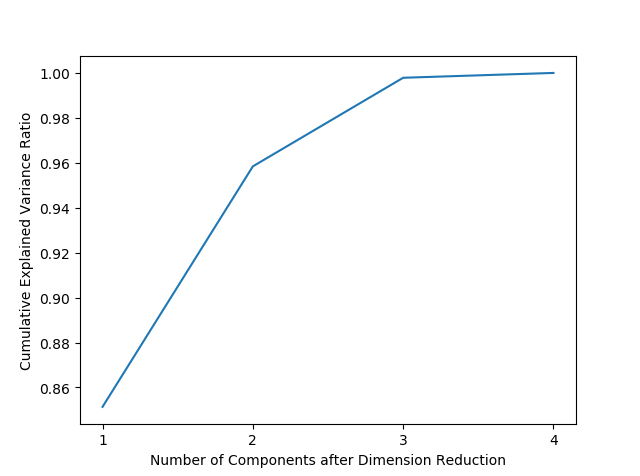
\includegraphics[width=0.35\textwidth]{Figure_2.png}\\
		\caption{累积可解释方差贡献率曲线}
	\end{figure}
	\subsubsection{代码内容分析}
	侯锐来写
	
	\subsubsection{优劣解距离法分析编程能力}
	
	\section{代码介绍}\label{sec3}
	\subsection{开源地址}
	
	\subsection{实现逻辑}
	\label{sec3:subsec2}

	
	\section{案例分析}\label{sec4}
	
	
	\section{意见和建议}\label{sec5}

	
	%===================================== 参考文献  ==========================================
	\section{参考文献}\label{sec:sec4}

	
\end{document}